\documentclass{beamer}
\usetheme{default} % no fancy navigation or anything ... 
\usefonttheme{serif}   
%\usepackage{lmodern}
\usepackage{svgcolor}
\usepackage{verbatim}
\usepackage[german]{babel}
%\usepackage[latin1]{inputenc}
\usepackage{shapepar}
\usepackage{graphicx}

\title     {\LaTeX{} Mini Intro}
\author    {Tobias Oetiker}
\institute {OETIKER+PARTNER AG}
\date      {It's only the Beginning!}

\begin{document}     
\begin{frame}
  \titlepage
\end{frame}

\begin{frame}
\begin{itemize}
\item \LaTeX{} Hintergrund
\item Funktionsprinzip
\item \LaTeX{}-Beispiele
\end{itemize}
\end{frame}

\begin{frame}[fragile]{\LaTeX Hintergrund}
\begin{itemize}
\item Professionelle Standard-Layouts (WYGLRG)
\item Satz mathematischer Formeln
\item Logisches \verb+\emph{+Mark-Up\verb+}+\\
      im Gegensatz zu optischem \underline{\textbf{\textrm{Mark-Up}}}
\item Inhaltsverzeichnis, Bibliographie, 
  Stichwortverzeichnis, Querverweise, Graphikeinbindung
\item Auf verschiedenen Plattformen frei verf�gbar.
\item Langzeitstabile Sprache (seit 1985).
\end{itemize}
\end{frame}

\begin{frame}{Funktionsprinzip}
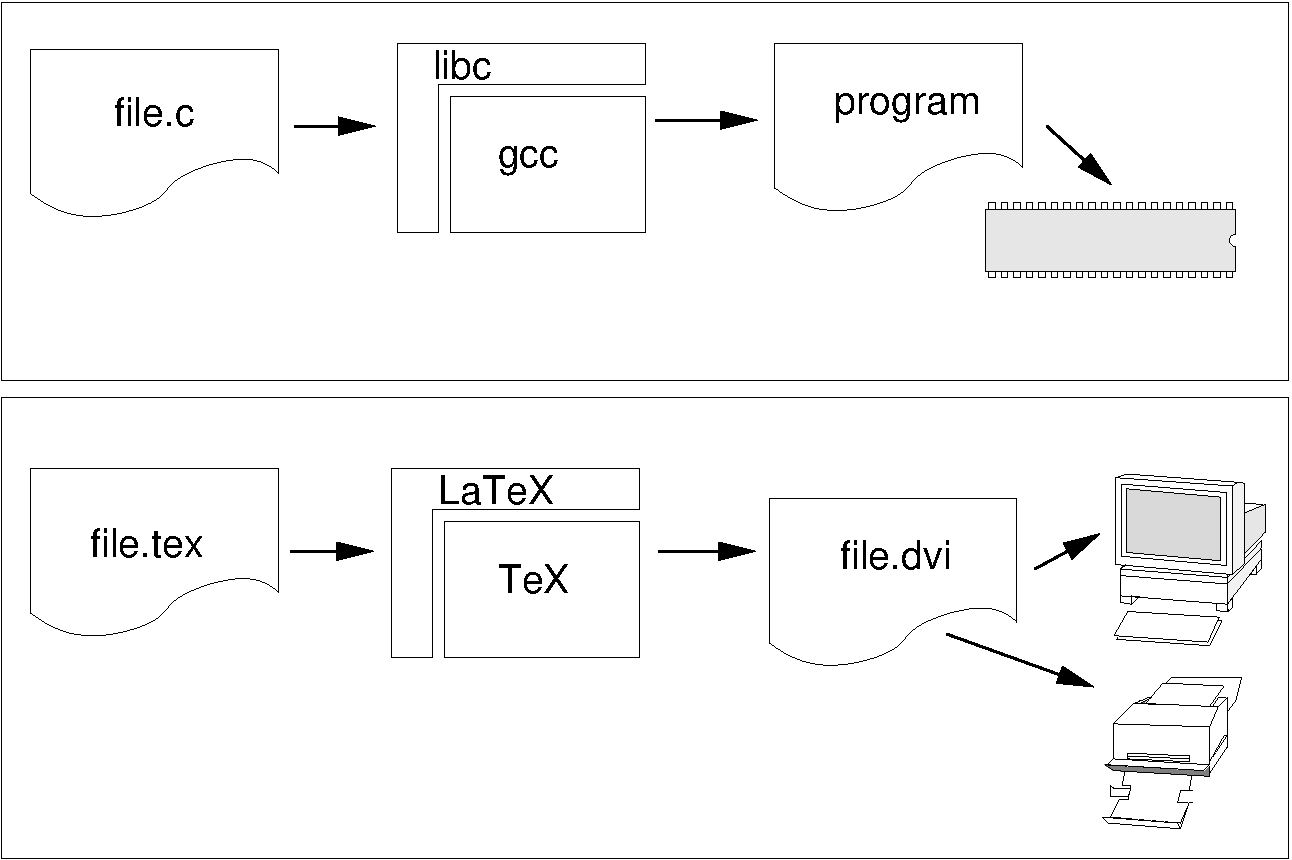
\includegraphics[width=\textwidth]{process}
\end{frame}

\begin{frame}[fragile]{Dokument}
\begin{verbatim}
\documentclass[a4paper]{article}
\usepackage[german]{babel}
\usepackage[latin1]{inputenc}
\begin{document}
\section{Ich bin Blindtex}
Von Geburt an. Es hat lange gedauert, bis ich
begriffen habe, was es bedeutet, ein blinder Text zu
sein: Man macht keinen Sinn. Man wirkt hier und da aus
dem Zusammenhang gerissen. Oft wird man gar nicht erst
gelesen ...

Aber ich bin gerne Text. Und sollten Sie mich jetzt
tats�chlich zu Ende lesen, dann habe ich etwas
geschafft, was den meisten
\end{document}
\end{verbatim}
\end{frame} 

\begin{frame}{Dokument Resultat}
\textbf{\large 1. Ich bin Blindtext}\\[1em]
        
Von Geburt an. Es hat lange gedauert, bis ich
begriffen habe, was es bedeutet, ein blinder Text zu
sein: Man macht keinen Sinn. Man wirkt hier und da aus
dem Zusammenhang gerissen. Oft wird man gar nicht erst
gelesen. Aber bin ich deshalb ein schlechter Text? Ich
weiss, dass ich nie die Chance haben werde im Stern zu
erscheinen. Aber bin ich darum weniger wichtig? Ich
bin blind!

\hspace*{1em}Aber ich bin gerne Text. Und sollten Sie
mich jetzt tats�chlich zu Ende lesen, dann habe ich
etwas geschafft, was den meisten
\end{frame}

\begin{frame}[fragile]{Mathematik}

\setlength{\fboxsep}{1em}
\begin{minipage}{0.5\textwidth}
\begin{verbatim}
\frac{1}
 {\alpha_{ij} + x^2}
\end{verbatim}
\end{minipage}\hspace{1cm}%
\framebox{\parbox{0.2\textwidth}{
\begin{displaymath}
\frac{1}
{\alpha_{ij} + x^2}
\end{displaymath}}}
\end{frame}

\begin{frame}{Mathematik II}
\begin{displaymath}
\frac{\prod _{n=1}^{\infty }(1-{x^{2 n}})}
  {\prod _{n=1}^{\infty}(1-{x^n})}
  =\sum _{k=-\infty }^{\infty }{x^{2 {k^2}+k}}
\end{displaymath}

\begin{displaymath}
\sqrt{6 + {\sqrt{6 + {\sqrt{6 + 
          {\sqrt{6 + {\sqrt{6 + 
                  {\sqrt{6 +  \cdots }}}}}}}}}}} = 3
\end{displaymath}
\end{frame}

\begin{frame}{It's only the Beginning!}

{\tiny
\heartpar{Die Gestalt des Herzens gleicht einem gut faustgro�en,
abgerundeten Kegel, dessen Spitze nach unten und etwas nach links vorne
weist. Das Herz sitzt beim Menschen in der Regel leicht nach links versetzt
hinter dem Brustbein (siehe weiter unten unter Topographie), in seltenen
F�llen nach rechts versetzt (die sogenannte Dextrokardie -
Rechtsherzigkeit), meist bei Situs inversus (spiegelverkehrter
Organanordnung).
Das gesunde Herz wiegt etwa 0,5\% des K�rpergewichts und im Durchschnitt
zwischen 300 und 350 g, wobei es bei dauerhafter Belastung eher mit der
(risikoarmen) Vergr��erung schon bestehender Herzmuskelzellen reagiert - ab
ca. 500 g, dem so genannten kritischen Herzgewicht, beginnt das Herz neben
strukturellen krankhaften Ver�nderungen bei regelm��ig auftretenden
Belastungssituationen ganz neue Herzmuskelzellen zu bilden, und es erh�ht
sich das Risiko einer absoluten Mangelversorgung der nunmehr gr��eren
Zellanzahl mit Sauerstoff, da die versorgenden Koronararterien nicht in
gleichem Ma�e mitwachsen.}}
\end{frame}

\begin{frame}{Try \LaTeX{} Online}
\url{http://www.scribtex.com}
\end{frame}

\end{document}

